\section{Обзор методов извлечения признаков на основе обучения без учителя}
\label{sec:Chapter2} \index{Chapter2}

В разделе \ref{sec:Chapter1} приведено описание данных методов. В этой главе рассмотрим детали трех перечисленных подходов.

\subsection{Barlow Twins}

Начнем обзор с метода Barlow Twins, который был предложен в июне 2021 года. Его архитектура представлена ниже на рисунке \ref{BT_arch}. Он достаточно нагляден и предлагает довольно эффективную реализацию вышеописанных задач. 

\begin{figure}[H]
        \center{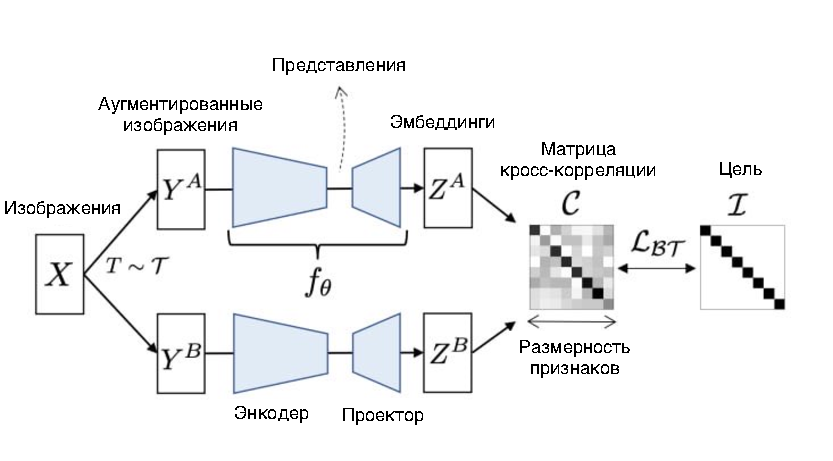
\includegraphics[height=8cm, keepaspectratio]{pictures/Barlow_Twins_arch.pdf}}
        \caption{Архитектура метода Barlow Twins}
        \label{BT_arch}
\end{figure} 

Для простоты понимания алгоритм работы метода можно разбить на три этапа. 

\subsubsection{Этап 1}

На вход поступает выборка объектов X. Объекты могут быть любые, в зависимости от конкретной задачи: тексты, геоданные, биологические данные. В данной работе многие этапы будут рассматриваться на примере изображений в качестве входных данных.

Для каждого объекта из исходной выборки создаются две разные аугментации, таким образом выборка подразделяется на две выборки $Y^A$ и $Y^B$, каждая из которых содержит аугментированные объекты из исходного набора.

Для изображений в качестве аугментаций как правило используются следующие преобразования:
\begin{itemize}
    \item Применяются всегда:
        \begin{enumerate} 
            \item Случайное кадрирование (random cropping);
            \item Изменение размера на $224\times224$ (resizing).
        \end{enumerate}
    \item Применяются с некоторыми вероятностями (одинаковыми для двух аугментаций):
        \begin{enumerate} 
            \item Зеркальное отображение по горизонтали (horizontal flipping);
            \item Color jittering;
            \item Преобразование в черно-белый формат (converting to grayscale).
        \end{enumerate}
    \item Применяются с некоторыми вероятностями (различными для  двух аугментаций):
        \begin{enumerate} 
            \item Размытие по Гауссу (Gaussian blurring);
            \item Соляризация (solarization).
        \end{enumerate}
\end{itemize}

Они используются конкретно в методе Barlow Twins и чаще всего в других методах тоже. Но стоит сказать, что для других методов аугментации могут и немного различаться. Например, могут использоваться не все из последних пяти перечисленных, или могут использоваться дополнительно и другие аугментации, такие как аффинные преобразования, фильтрация Собеля и тд.

\subsubsection{Этап 2}

Далее каждая из выборок подается на вход нейронной сети, обозначенной как $f_\theta$. Она состоит из двух частей: энкодера и проектора. Для преобразования изображений в качестве энкодера обычно используются архитектура сети ResNet-50 \cite{ResNet} без последнего слоя классификации (2048 нейронов на выходе). Далее следует нейронная сеть проектора. В Barlow Twins она состоит из трех полносвязных слоев, каждый из которых имеет выход 8192 нейрона. После первого и второго слоя проектора идет слой Batch Normalization. 

На выходе из энкодера мы получаем векторы, которые как раз и называются представлениями. А векторы, полученные на выходе из проектора, будем называть эмбедингами. Здесь важно отметить: разница в том, что представление - это и есть наш целевой вектор, который далее мы будем использовать для практических задач, а эмбединги мы передаем в функцию потерь, то есть используем их исключительно для обучения нейронной сети. В данном методе проектор используется для того, чтобы немного расширить признаковое пространство и далее работать с большей размерностью.

\subsubsection{Этап 3}

Итак, мы получили две выборки, состоящие из эмбедингов, обозначенные как $Z^A$ и $Z^B$. Мы составляем для них матрицу кросс-корреляции, элементы которой считаются по следующей формуле: 
$$
c_{ij}=\frac{\sum_b z_{ib}^A z_{bj}^B}
{\sqrt{\sum_b (z_{ib}^A)^2} \sqrt{\sum_b (z_{bj}^B)^2}}
$$
здесь $b=\overline{1,N}$, где N - количество элементов в исходной выборке, $i, j=\overline{1,M}$, где M - размерность эмбедингов в выборках $Z^A$, $Z^B$.

Далее мы применяем функцию потерь, которая выглядит следующим образом:
$$
L_{BT}=\sum_{i}(1-c_{ii})^2+\lambda\sum_{i}\sum_{j\neq i}c_{ij}^2
$$
где $\lambda$ - положительный гиперпараметр, введенный для регуляризации второго слагаемого функции.

Как можем видеть, цель данной функции - приблизить нашу матрицу кросс-корреляции к единичной матрице. Минимизируя первое слагаемое, мы устремляем диагональные элементы матрицы к единице. В результате чего все положительные пары эмбедингов должны коррелировать друг с другом, что обеспечивает их инвариантность. Таким образом выполняется первая задача, описанная в разделе \ref{sec:methods}. Минимизируя второе слагаемое функции, мы устремляем недиагональные элементы матрицы к нулю, тем самым декоррелируя пространство признаков внутри каждого эмбединга. И теперь уже выполнена и вторая задача.

Как видим, Barlow Twins эффективно решает две задачи, совмещая их в функции потерь. В последующих разделах все рассмотренные методы будут оцениваться на практических задачах. Соответственно, данный метод, как и другие нижеописанные, еще будет упоминаться, а также сравниваться друг с другом.

\subsection{Whitening MSE}

Метод Whitening-MSE был предложен чуть раньше метода Barlow Twins, в мае 2021 года. Он использует другие, но не менее интересные подходы для реализации двух описанных задач.

\begin{figure}[H]
        \center{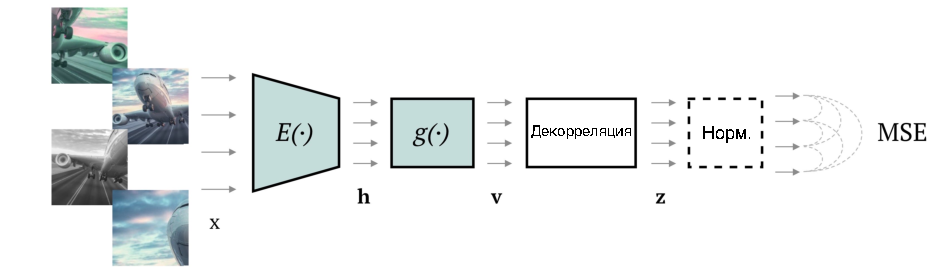
\includegraphics[height=4.5cm, keepaspectratio]{pictures/W_MSE_arch.pdf}}
        \caption{Архитектура метода Whitening-MSE}
        \label{W_MSE_arch}
\end{figure} 

Первый этап данного метода аналогичен методу Barlow Twins. Разница заключается только в том, что W-MSE предполагает любое количество аугментаций для каждого объекта выборки, тем самым увеличивая количество положительных пар в наборе.

Второй этап тоже аналогичен. Различаются только архитектуры проекторов. Проектор W-MSE состоит всего из одного полносвязного слоя, который имеет 1024 нейрона на выходе. За ним следует слой Batch Normalization. Здесь наоборот необходимо сузить размерность признакового пространства для успешного выполнения последующих преобразований.

Далее, в отличие от метода Barlow Twins, данный метод имеет дополнительный этап, который в англоязычных источниках называется Whitening. Мы для упрощения будем называть его декорреляцией. 

Итак, на выходе из проектора g(x) мы получаем выборку из $N\times d$ эмбедингов, где N - количество объектов в исходной выборке, d - количество аугментаций для каждого объекта. Пусть $K=N\times d$. Тогда для каждого из эмбедингов $v$ мы применяем следующее преобразование:
$$
Whitening(v)=W_v(v-\mu_v)
$$

Здесь:
\begin{itemize}
    \item $\mu_v$ - вектор, рассчитанный как среднее значение по выборке: $\mu_v=\frac{1}{k}\sum_kv_k$ ;
    \item $W_v$ - такая матрица, что: $W_vW_v^T=\Sigma_v^{-1}$, где $\Sigma_v$- матрица ковариации:
    $$
    \Sigma_v=\frac{1}{K-1}\sum_k(v_k-\mu_k)(v_k-\mu_k)^T.
    $$
\end{itemize} 

Для вычисления матрицы $W_v$ используется разложение Холецкого.
Данное разложение позволяет посчитать для любой симметричной положительно определенной матрицы A матрицу L, такую что $A=LL^T$, где L - нижняя треугольная матрица со строго положительными элементами на диагонали. Можно также записать разложение в эквивалентной форме: $A=U^TU$, где U - верхняя треугольная матрица со строго положительными элементами на диагонали. 

Разложение Холецкого всегда существует и единственно для любой симметричной положительно определённой матрицы. Наша матрица $\Sigma_v$ удовлетворяет этим критериям, поэтому мы всегда сможем найти матрицу $W_v$.

В результате данных преобразований мы получаем новую выборку $Z=\{z_1, \dots, z_K\}$, $z_i=Whitening(v_i)$, $i=\overline{1,K}$, в которой декоррелированo пространство признаков внутри каждого эмбединга. Таким образом мы выполнили задачу декорреляции.

Далее, переходя к последнему этапу, мы передаем выборку $Z$ в функцию потерь, которая выглядит следующим образом:
$$
L_{W\_MSE}=\frac{2}{Nd(d-1)}\sum dist(z_i, z_j)
$$
где $dist(z_i, z_j)$ - расстояние между положительными парами $z_i$ и $z_j$:
$$
dist(z_i, z_j)=\left\|\frac{z_i}{\|z_i\|_2}-\frac{z_j}{\|z_j\|_2}\right\|_2^2
$$
N и d - как уже говорилось ранее, количество объектов в исходной выборке и количество аугментаций, тогда:
\begin{itemize}
    \item $\frac{d(d-1)}{2}$ - количество положительных пар для каждого объекта;
    \item $\frac{Nd(d-1)}{2}$ - общее количество положительных пар в наборе.
\end{itemize} 

С помощью данной функции потерь мы минимизируем среднее значения расстояния между полученными эмбедингами для всех положительных пар набора. То есть мы требуем, чтобы положительные представления находились близко друг к другу в общем пространстве представлений. Данное условие выполняет первую задачу инвариантности.

\subsection{VICReg}

Метод VICReg (Variance-Invariance-Covariance Regularization) очень похож на метод Barlow Twins. Он заимствует оттуда механизм декорреляции, однако использует более усовершенствованную функции потерь и другой подход для сохранения инвариантности.

\begin{figure}[H]
        \center{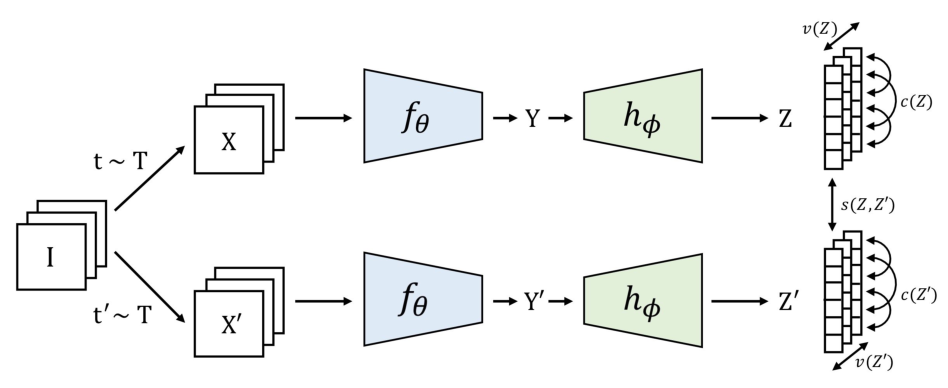
\includegraphics[height=6cm, keepaspectratio]{pictures/VICReg_arch.pdf}}
        \caption{Архитектура метода VICReg}
        \label{VICReg_arch}
\end{figure} 

Первые да этапа полностью аналогичны методу Barlow Twins, архитектура проектора полностью совпадает. Поэтому перейдем сразу к последнему этапу и рассмотрим функцию потерь.

Итак, мы получили две выборки эмбедингов Z и Z'. Для них мы рассчитываем следующую функцию потерь:
$$
L_{VICReg}=\sum_{i\in D}\sum_{t'\in T} \left[\lambda s(Z, Z')+\mu\{v(Z)+v(Z')\}+\nu\{c(Z)+c(Z')\}\right]
$$

здесь $D$ - исходная выборка, $T$ - примененные аугментации, $\lambda$, $\mu$, $\nu$ - положительные гиперпараметры, введенные для регуляризации каждого из слагаемых функции.

Данная функция является композицией трех функций: 
\begin{itemize}
    \item $v(Z)$ - дисперсия;
    \item $s(Z, Z')$ - инвариантность;
    \item $c(Z)$ - ковариация.
\end{itemize}

Разберем каждую функцию по отдельности. Пусть N - количество объектов в исходной выборке, d - размерность полученных эмбедингов в выборках Z, Z'. Также для удобства введем матрицу Z, которая составляется для каждой из выборок:
\begin{figure}[H]
        \center{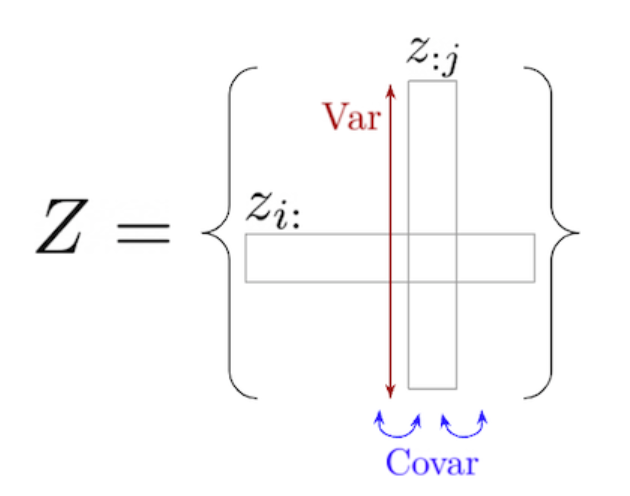
\includegraphics[height=5cm, keepaspectratio]{pictures/emb_matrix.png}}
        % \caption{Пример актуальной проблемы.}
        \label{ris:image}
\end{figure}
В строках данной матрицы содержатся эмбединги $z_i$, $i=\overline{1, N}$, а в столбцах признаки $z_j$, $i=\overline{1, d}$. Таким образом, размерность матрицы: $N\times d$.

Начнем с дисперсии. Введем следующую функцию:
$$
Var(z_j)=\frac{1}{n-1}\sum_{i=1}^N(z_{ij}-\overline{z_{j}})^2
$$

здесь $\overline{z_{j}}=\frac{1}{n}\sum_{i=1}^Nz_{ij}$ - среднее значение вектора $z_j$, $j=\overline{1, d}$, которое рассчитывается для каждого признака. Как видим, функция $Var(z_j)$ считает для каждого признака значение дисперсии.

Тогда функция $v(Z)$ выглядит следующим образом:
$$
v(Z)=\frac{1}{d}\sum_{j=1}^dmax\left(0, \gamma - \sqrt{Var(z_j)+\epsilon}\right)
$$

Цель данной функции заключается в том, чтобы сделать среднеквадратичное отклонение для каждого признака выборки превышающим значение некоторого гиперпараметра $\gamma$. Функция $v(Z)$ используется исключительно для дополнительного предотвращения проблемы коллапса, поскольку порог среднеквадратичного отклонения не позволит модели генерировать константные выходы. 

Функция инвариантности $s(Z, Z')$ выглядит следующим образом:
$$
s(Z, Z')=\frac{1}{n}\sum_i\|z_i-z_i'\|_2^2
$$

Цель данной функции, как и в W-MSE, сохранить инвариантность представлений, за счет минимизации расстояния между положительными парами. Здесь используется более простая функция: евклидова метрика. Таким образом мы решаем первую задачу. 

Рассмотрим теперь функцию ковариации. Для этого введем матрицу ковариции: 
$$
C(Z)=\frac{1}{n-1}\sum_{i=1}^N(z_i-\overline{z})(z_i-\overline{z})^T
$$

где 
$
\overline{z}=\frac{1}{n}\sum_{i=1}^Nz_{i}
$  
- среднее значение вектора по выборке.

Тогда функция $c(Z)$ имеет вид:
$$
c(Z)=\frac{1}{d}\sum_{l\neq m}C(Z)_{lm}^2
$$

Цель функции $c(Z)$ - приблизить все недиагональные элементы матрицы ковариции $C(Z)$ к нулю. С помощью этого мы декоррелируем признаковое пространство внутри эмбедингов, тем самым выполняя вторую задачу.

\subsection{Оценка и сравнение рассмотренных методов}
\label{Eval}

Оценим результаты работы методов на задаче классификации изображений из набора ImageNet. Для оценивания использовалось два способа: линейная оценка, оценка частичного обучения. 

Линейная оценка проводится следующим образом:
\begin{enumerate}
    \item Обучаем модель для задачи извлечения признаков, назовем ее "базовая сеть";
    \item Дописываем линейный классификатор, принимающий на вход представления из базовой сети;
    \item Замораживаем базовую сеть;
    \item Дообучаем только линейный классификатор на полном наборе размеченных данных.
\end{enumerate} 

Оценка частичного обучения проводится следующим образом:
\begin{enumerate}
    \item Обучаем модель для задачи извлечения признаков;
    \item Дописываем линейный классификатор, принимающий на вход представления из базовой сети;
    \item Дообучаем базовую сеть и линейный классификатор на неполном наборе размеченных данных.
\end{enumerate} 

В таблице представлена точность Top-1 и Top-5. А также процент размеченных данных, используемых для частичного обучения.

\begin{center}
\begin{tabular}{ l c c c c c c c } 
  \hline
  \multirow{3}{4em}{Метод} & \multicolumn{2}{c}{Линейная оценка} & & \multicolumn{4}{c}{Частичное обучение} \\
  \cline{2-3}\cline{5-8}
  
  & Top-1 & Top-5 & &  \multicolumn{2}{c}{Top-1} &  \multicolumn{2}{c}{Top-5}  \\ 
  & & & & 1\% & 10\% & 1\% & 10\% \\ 
  \hline
  
  Обучение с учителем & 76.5 & - & & 25.4 & 56.4 & 48.4 & 80.4 \\
  \hline

  MoCo \cite{MoCo} & 60.6 & - & & - & - & - & - \\
  SimCLR \cite{SimCLR} & 69.3 & 89.0 & & 48.3 & 65.6 & 75.5 & 87.8 \\
  MoCo V2 \cite{MoCo_V2} & 71.1 & 90.1 & & - & - & - & - \\
  W-MSE 4 \cite{Whitening_MSE} & 69.4 & - & & - & - & - & - \\
  Barlow Twins \cite{Barlow_Twins} & 73.2 & 91.0 & & $\underline{55.0}$ & $\underline{69.7}$ & 79.2 & 89.3 \\
  VICReg \cite{Vicreg} & $\underline{73.2}$ & $\underline{91.1}$ & & 54.8 & 69.5 & $\underline{79.4}$ & $\underline{89.5}$ \\
  
  \hline
\end{tabular}
\end{center}

Для всех методов в таблице использовалась архитектура ResNet-50 \cite{ResNet} в качестве энкодера. Обучение базовой сети проводилось на 1000 эпохах. Для линейной оценки дообучение проводилась на 100 эпохах, для оценки частичного обучения - на 20 эпохах. Для обоих оценок размер пакета составлял 256.

В таблице подчеркнуты лучшие результаты. Как можем видеть, лидируют методы на основе обучения без учителя, в частности Barlow Twins \cite{Barlow_Twins} и VICReg \cite{Vicreg}.